\documentclass{article}
\usepackage{blindtext}
\usepackage{amsmath}
\usepackage[spanish]{babel}
\usepackage[T1]{fontenc}
\usepackage{float}
\usepackage{geometry}
 \geometry{
 a4paper,
 total={170mm,257mm},
 left=20mm,
 top=20mm,
 }
\title{Informe: Estudio del apego emocional al propio país y a Europa}
\author{Mariona Puente Quera}
\date{2024-07-24}

\usepackage{Sweave}
\begin{document}
\maketitle
\Sconcordance{concordance:Informe.tex:Informe.Rnw:1 17 1 1 0 3 1 1 6 1 5 7 0 2 2 1 0 %
4 1 3 0 1 2 20 1 1 33 1 2 19 1 1 34 1 2 1 34 1 2 23 1 1 34 1 2 1 34 1 2 %
1 34 1 2 1 34 1 2 1 34 1 2 31 1 1 34 1 2 1 34 1 2 1 34 1 2 1 34 1 2 1 %
34 1 2 1 34 1 2 1 34 1 2 1 34 1 2 1 34 1 2 1 34 1 2 1 34 1 2 1 34 1 2 1 %
34 1 2 44 1}



\begin{Schunk}
\begin{Sinput}
> if(!require(tinytex)){
+   install.packages('tinytex')
+   library(tinytex)
+ }
\end{Sinput}
\end{Schunk}

\begin{Schunk}
\begin{Sinput}
> tinytex::tlmgr_install('blindtext')
> tinytex::tlmgr_install('amsmath')
> tinytex::tlmgr_install("babel-spanish")
> tinytex::tlmgr_install("grfext")
> tinytex::tlmgr_install("float")
\end{Sinput}
\end{Schunk}

\section*{Objetivos iniciales}
Los objetivos propuestos inicialmente en el proyecto son los siguientes:

\begin{itemize}
    \item \textbf{OBJETIVO GENERAL:} Estudiar cómo correlacionan el apego emocional al propio país y el apego emocional a Europa, y el efecto del género, de la edad y de la nacionalidad en dicha correlación.
    \item \textbf{OBJETIVOS ESPECÍFICOS:}
    \begin{enumerate}
        \item Estudiar y visualizar cómo correlacionan el apego emocional al propio país y el apego emocional a Europa en nuestra muestra.
        \item Estudiar y visualizar los efectos de la variable género en dicha correlación.
        \item Estudiar y visualizar los efectos de la variable edad en dicha correlación.
        \item Estudiar y visualizar los efectos de la variable nacionalidad en dicha correlación.
        \item Estudiar y visualizar cómo correlacionan el apego emocional al propio país y el apego emocional a Europa entre diferentes subgrupos a escoger de entre los diferentes niveles de nuestras variables demográficas.
    \end{enumerate}
\end{itemize}
Con tal de analizar los resultados proporcionados por el dashboard estudiaremos cada objetivo específico por separado a continuación.

\section*{Resultados:}

\section{Estudiar y visualizar cómo correlacionan el apego emocional al propio país y el apego emocional a Europa en nuestra muestra.}

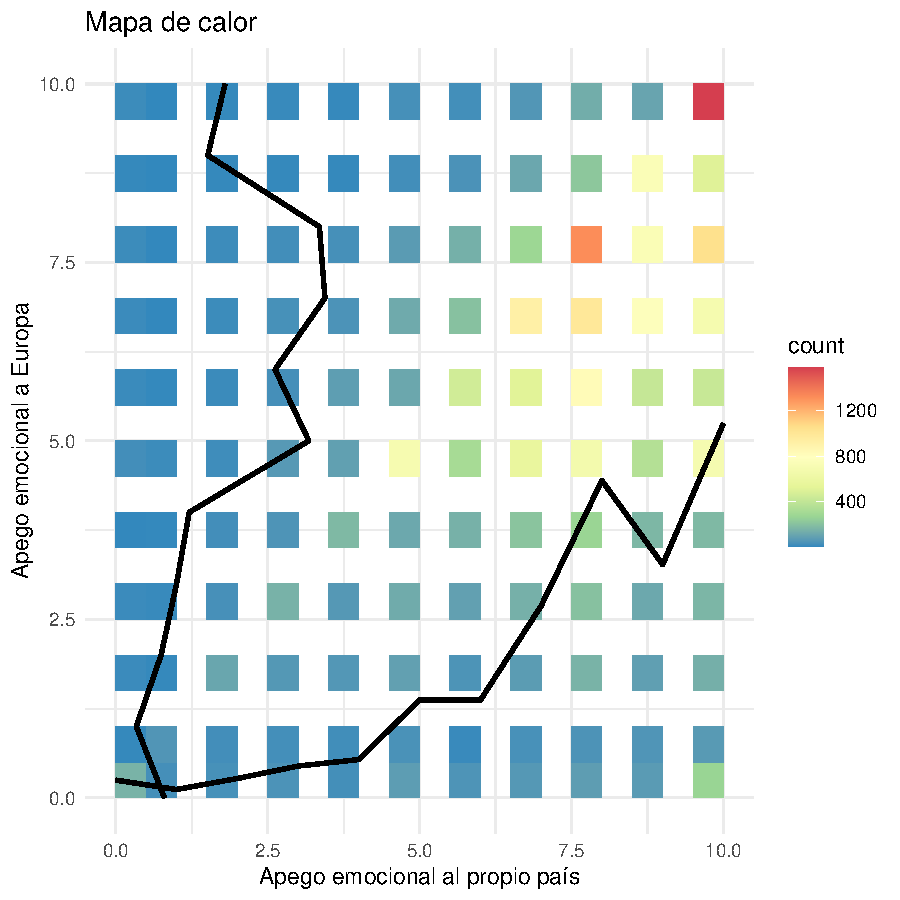
\includegraphics{Informe-004}

\section{Estudiar y visualizar los efectos de la variable género en dicha correlación.}
 \begin{itemize}
 \item D.E. = Desviación estándard
 \item AEPP = Apego emocional al propio país
 \item AEE = Apego emocional a Europa
 \end{itemize}
 \begin{table}[h!]
 \caption{Variable género}
 \begin{tabular}{l | c c c c c}
 \hline
 \bf{Género} & \bf{Media 'AEPP'} & \bf{D.E. 'AEPP'} & \bf{Media 'AEE'} & \bf{D.E. 'AEE'} & \bf{CORR. PEARSON} \\
 \hline
 Mujeres & 7.837861 & 2.145087 & 6.270493 & 2.471481 & 0.4100358 \\
 Hombres & 7.693225 & 2.21015 & 6.097755 & 2.525251 & 0.4146855 \\
 Tod@s & 7.770864 & 2.176612 & 6.190264 & 2.498028 & 0.4128778 \\
 \hline
 \end{tabular}
 \end{table}

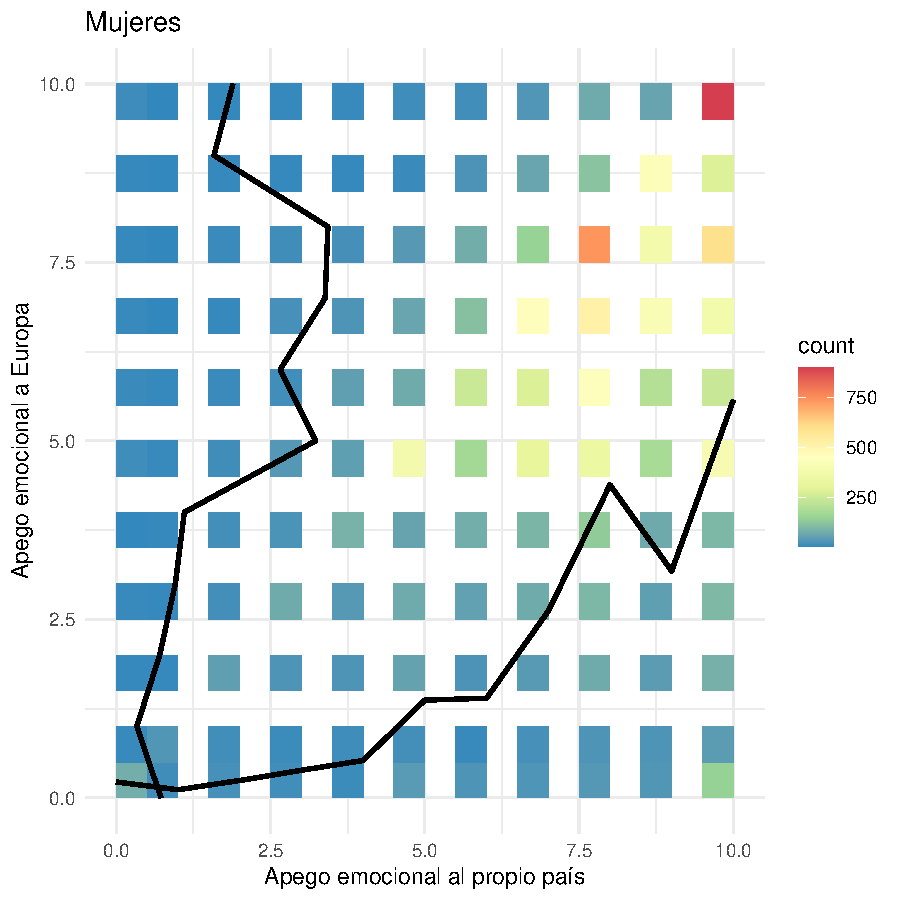
\includegraphics{Informe-005}

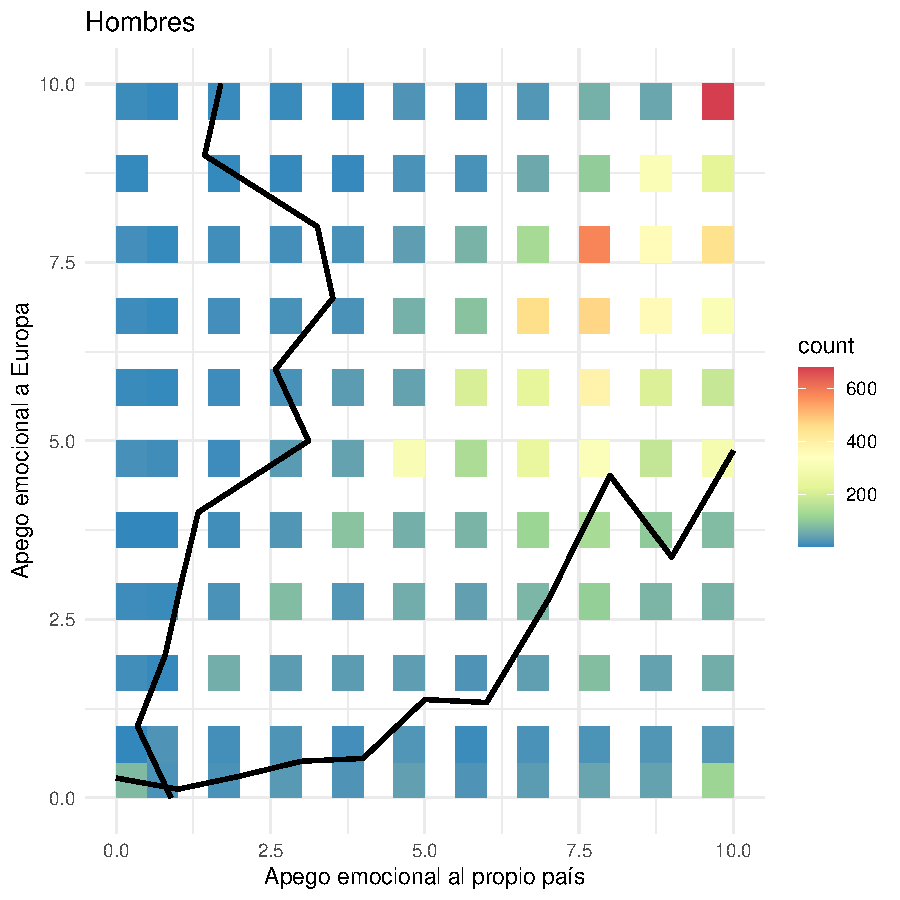
\includegraphics{Informe-006}

\newpage
\section{Estudiar y visualizar los efectos de la variable edad en dicha correlación.}
 \begin{itemize}
 \item D.E. = Desviación estándard
 \item AEPP = Apego emocional al propio país
 \item AEE = Apego emocional a Europa
 \end{itemize}
 \begin{table}[h!]
 \caption{Variable edad}
 \begin{tabular}{l | c c c c c}
 \hline
 \bf{Rango edad} & \bf{Media 'AEPP'} & \bf{D.E. 'AEPP'} & \bf{Media 'AEE'} & \bf{D.E. 'AEE'} & \bf{CORR. PEARSON} \\
 \hline
 Menores de 30 & 6.926075 & 2.360681 & 6.121974 & 2.354955 & 0.4800369 \\
 Entre 30 y 44 & 7.462656 & 2.19397 & 6.107612 & 2.466652 & 0.4444008 \\
 Entre 45 y 59 & 7.806323 & 2.102556 & 6.191416 & 2.490652 & 0.395468 \\
 Entre 60 y 74 & 8.161118 & 2.020955 & 6.27193 & 2.535688 & 0.3987813 \\
 75 o mayores & 8.466388 & 1.950735 & 6.222835 & 2.643745 & 0.3832552 \\
 Tod@s & 7.770864 & 2.176612 & 6.190264 & 2.498028 & 0.4128778 \\
 \hline
 \end{tabular}
 \end{table}
 
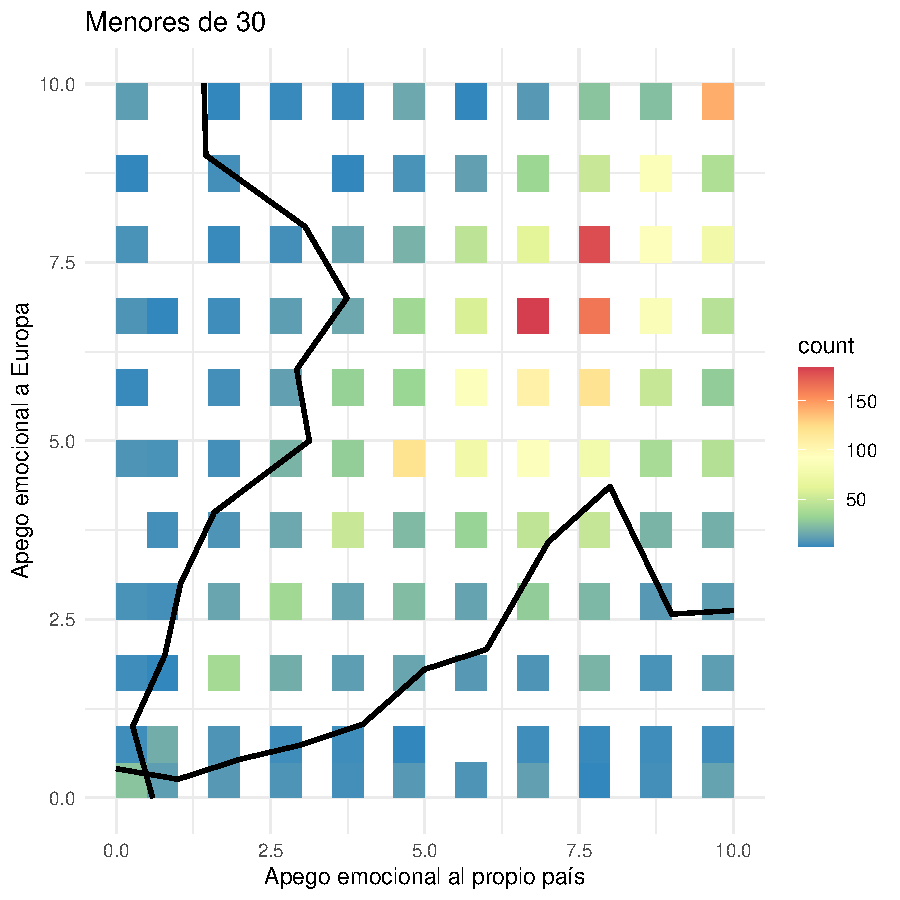
\includegraphics{Informe-007}

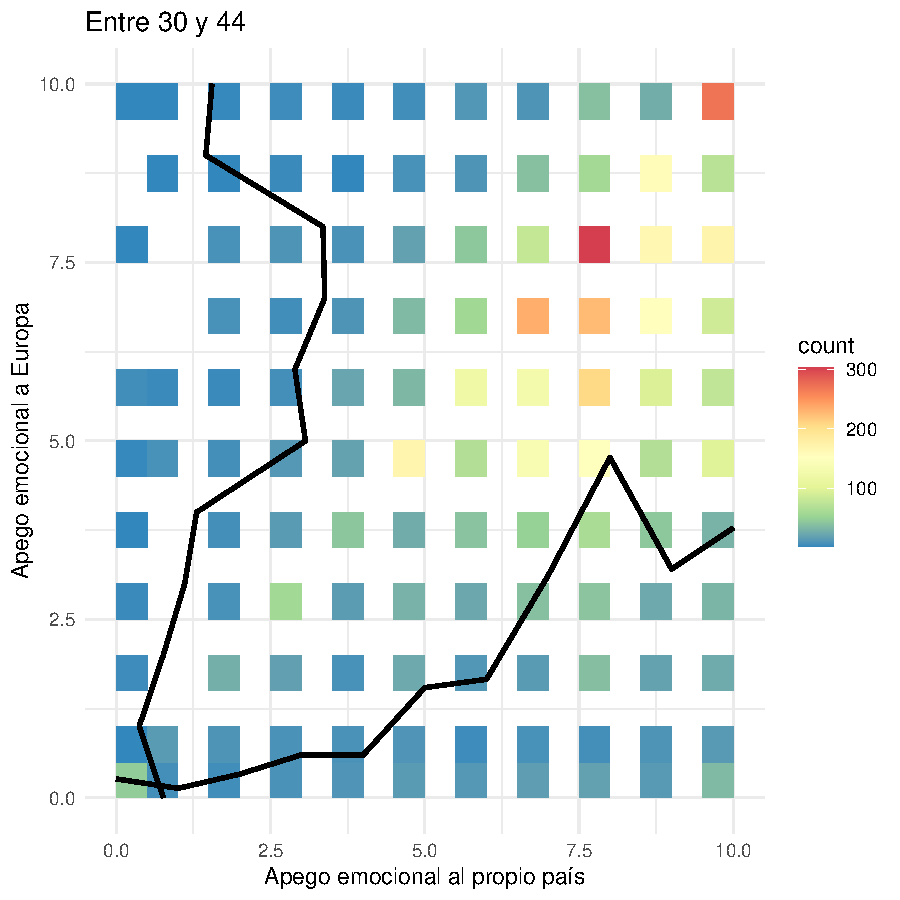
\includegraphics{Informe-008}

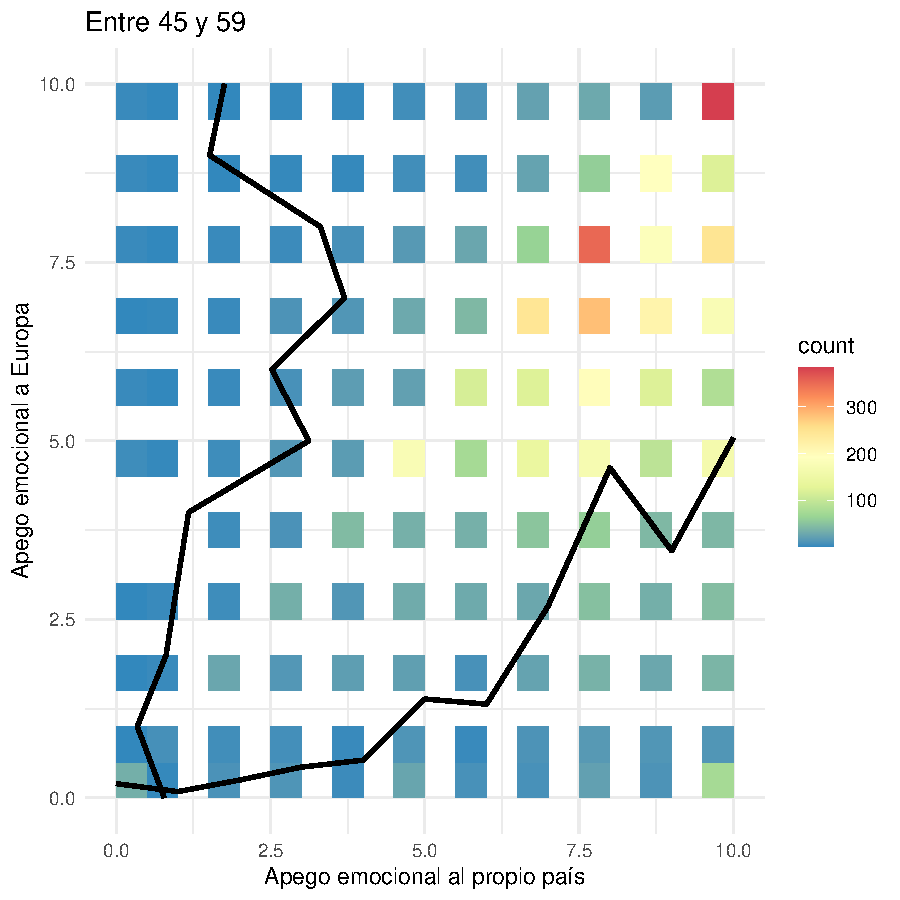
\includegraphics{Informe-009}

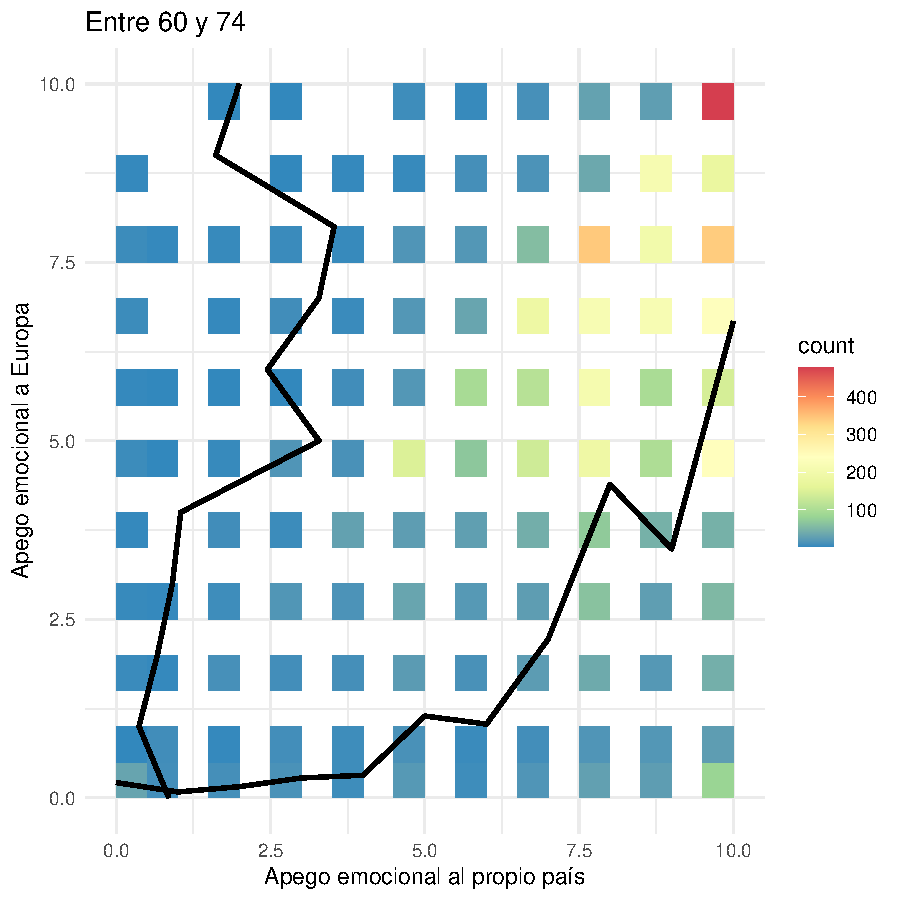
\includegraphics{Informe-010}

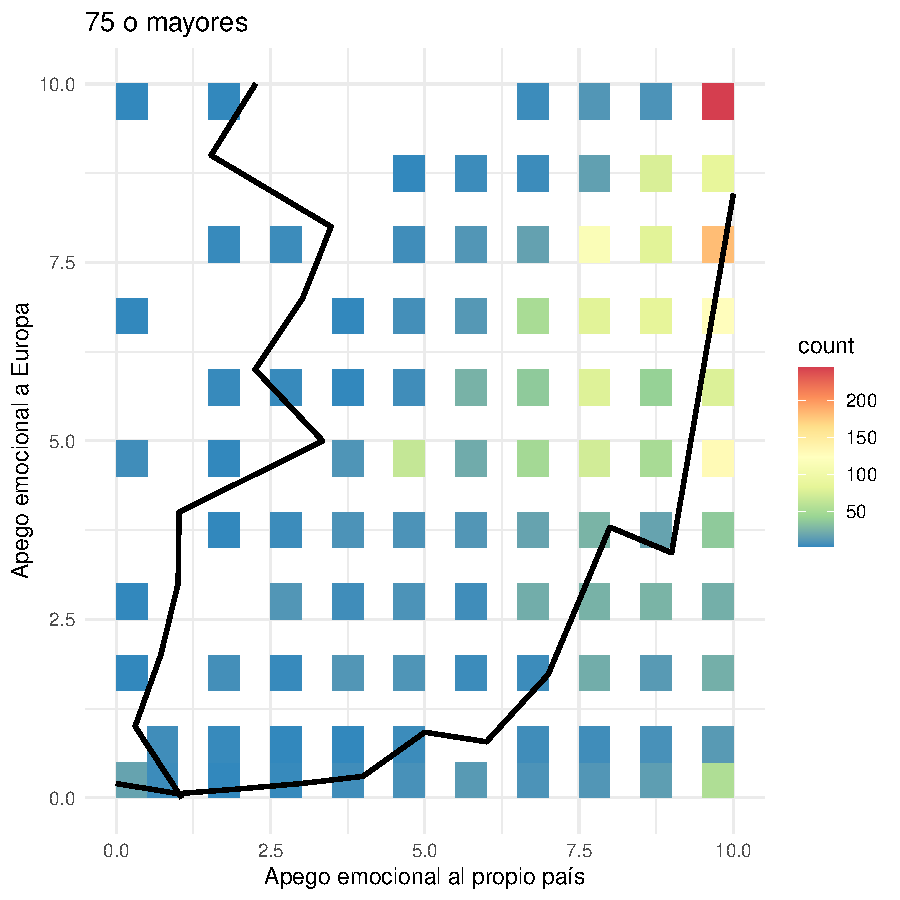
\includegraphics{Informe-011}

\newpage
\section{Estudiar y visualizar los efectos de la variable nacionalidad en dicha correlación.}
 \begin{itemize}
 \item D.E. = Desviación estándard
 \item AEPP = Apego emocional al propio país
 \item AEE = Apego emocional a Europa
 \end{itemize}
 \begin{table}[h!]
 \caption{Variable nacionalidad}
 \begin{tabular}{l | c c c c c}
 \hline
 \bf{País} & \bf{Media 'AEPP'} & \bf{D.E. 'AEPP'} & \bf{Media 'AEE'} & \bf{D.E. 'AEE'} & \bf{CORR. PEARSON} \\
 \hline
 Alemania & 7.212096 & 2.234437 & 6.486509 & 2.356144 & 0.5506882 \\
 Áustria & 8.36 & 1.829636 & 6.524541 & 2.3696 & 0.2826011 \\
 Croacia & 7.798714 & 2.247549 & 5.990909 & 2.59227 & 0.4341063 \\
 Eslovaquia & 7.570231 & 2.426643 & 5.966878 & 2.792222 & 0.4622578 \\
 Eslovenia & 7.753017 & 2.212389 & 5.930138 & 2.597684 & 0.458533 \\
 Finlandia & 8.630198 & 1.56143 & 6.838132 & 1.964155 & 0.3117515 \\
 Hungría & 8.167143 & 2.017117 & 7.1415 & 2.386804 & 0.4656425 \\
 Irlanda & 7.968688 & 1.918663 & 5.943641 & 2.399126 & 0.3305107 \\
 Lituania & 7.807777 & 2.296271 & 5.890895 & 2.731617 & 0.2824732 \\
 Noruega & 8.405101 & 1.668298 & 6.596847 & 2.154182 & 0.3667099 \\
 Países Bajos & 6.894737 & 2.092995 & 5.722584 & 2.187825 & 0.4928814 \\
 Reino Unido & 6.575758 & 2.731243 & 4.795679 & 2.788772 & 0.2884089 \\
 Suiza & 7.926705 & 1.826457 & 6.066909 & 2.297686 & 0.297761 \\
 Tod@s & 7.770864 & 2.176612 & 6.190264 & 2.498028 & 0.4128778 \\
 \hline
 \end{tabular}
 \end{table}

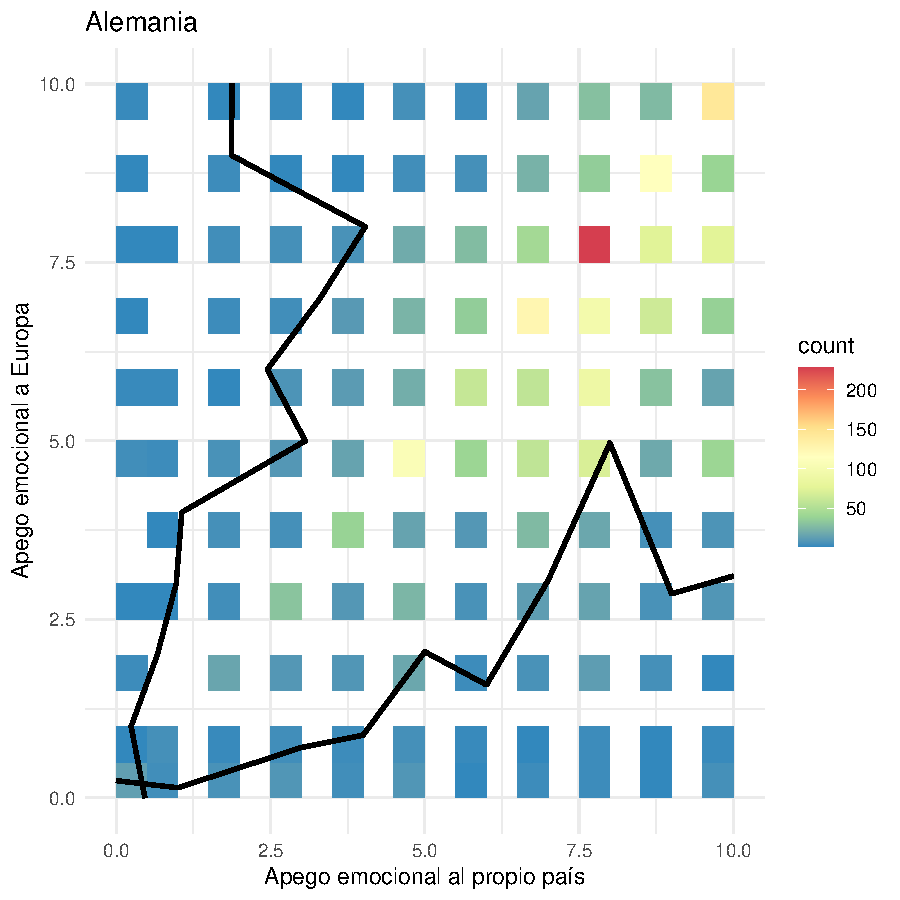
\includegraphics{Informe-012}

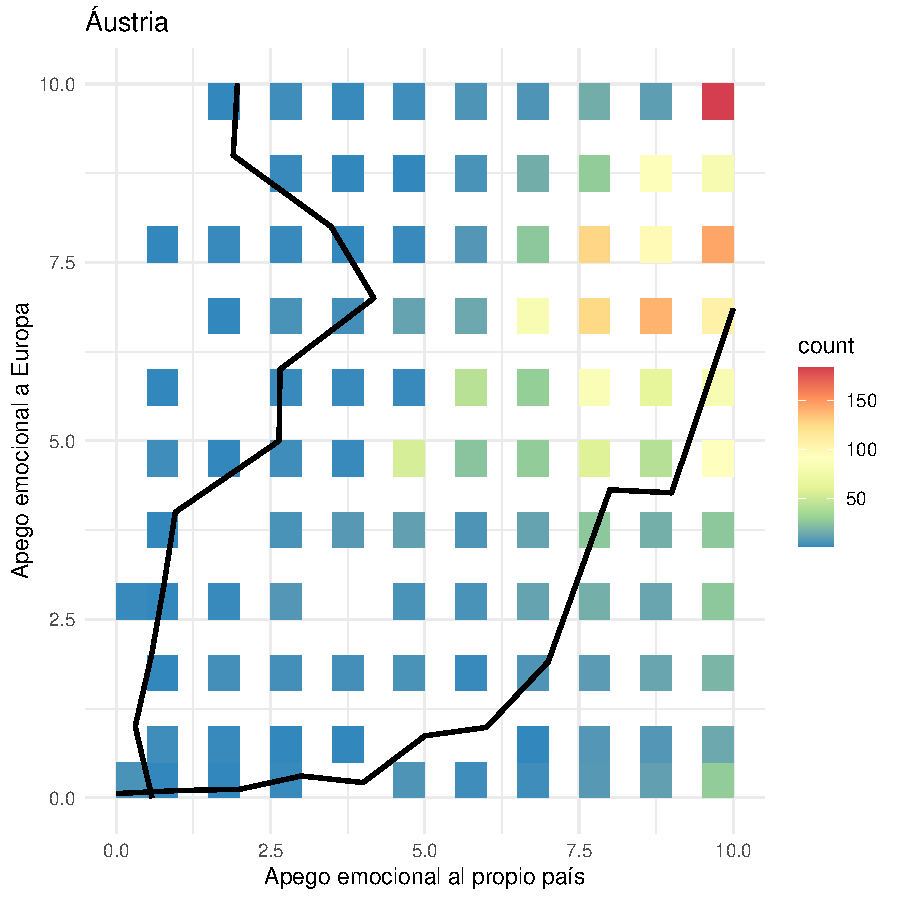
\includegraphics{Informe-013}

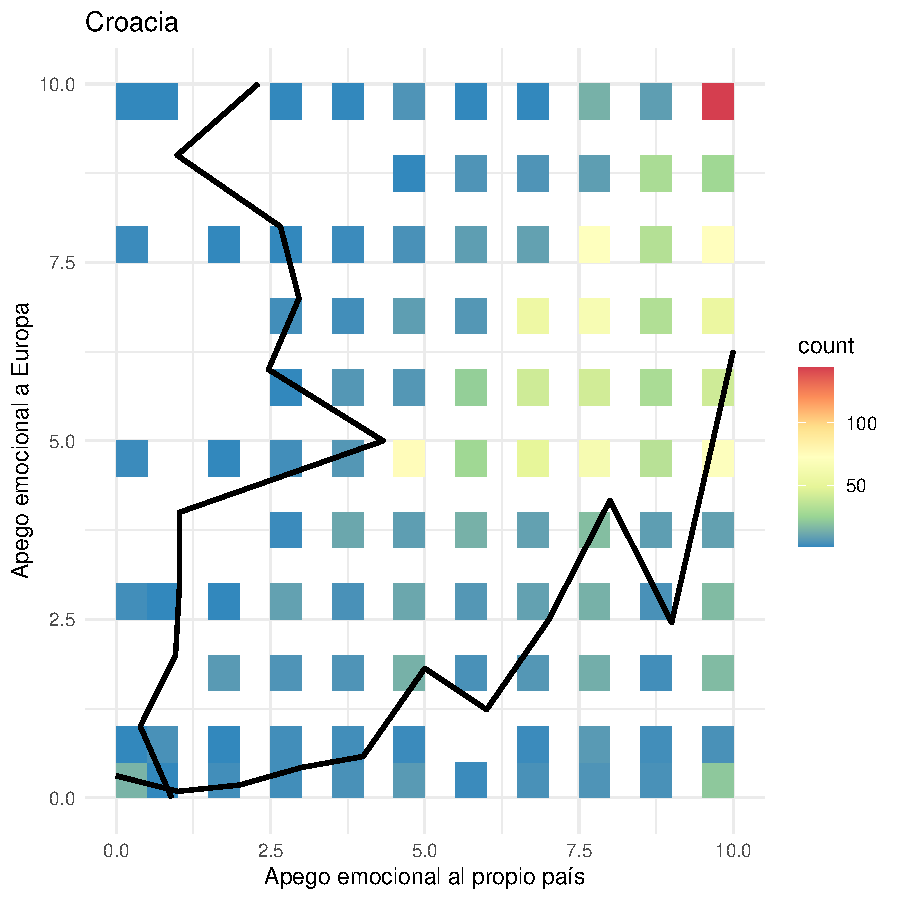
\includegraphics{Informe-014}

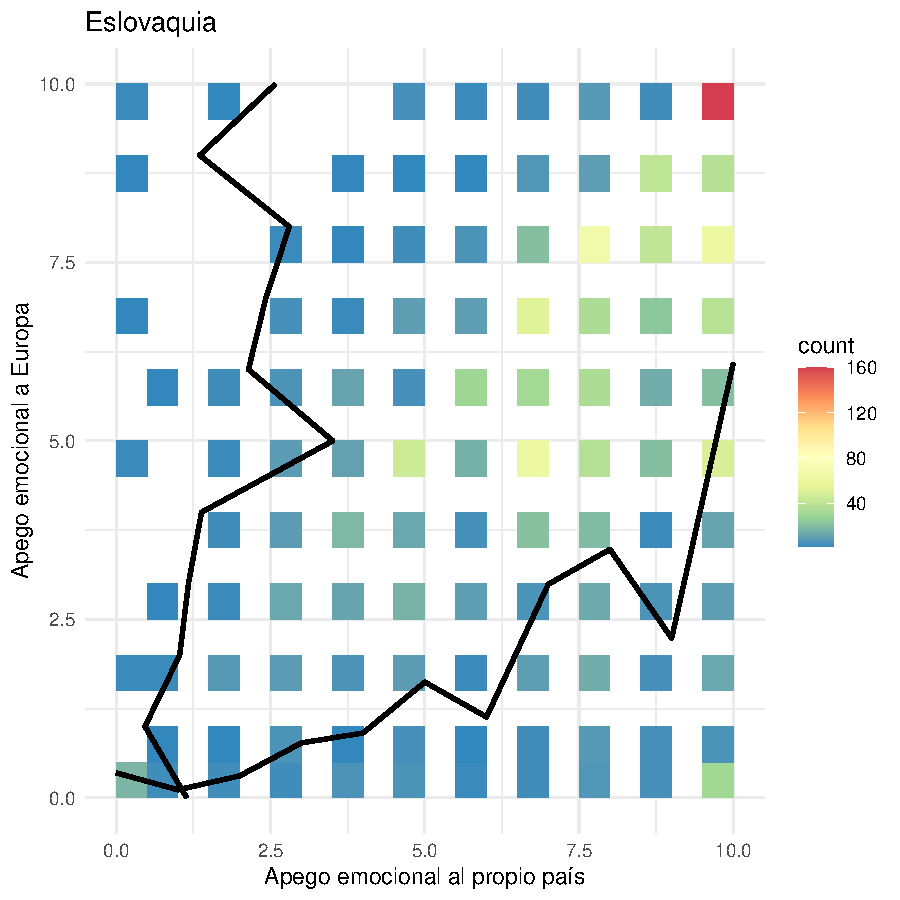
\includegraphics{Informe-015}

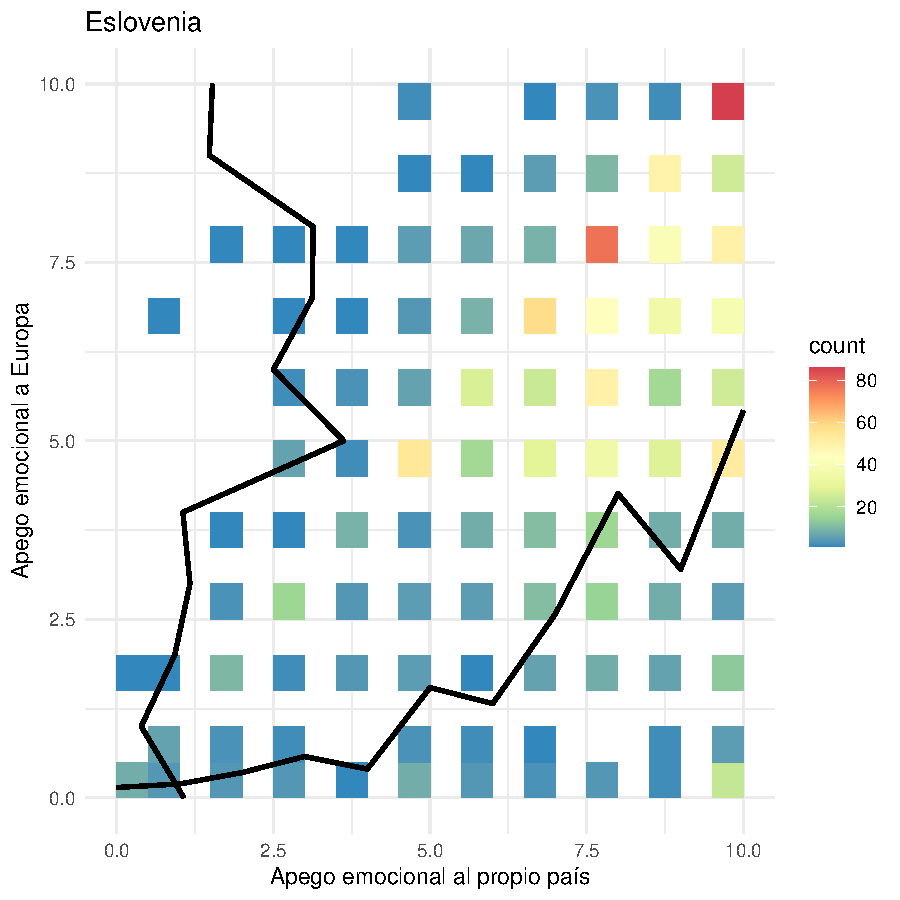
\includegraphics{Informe-016}

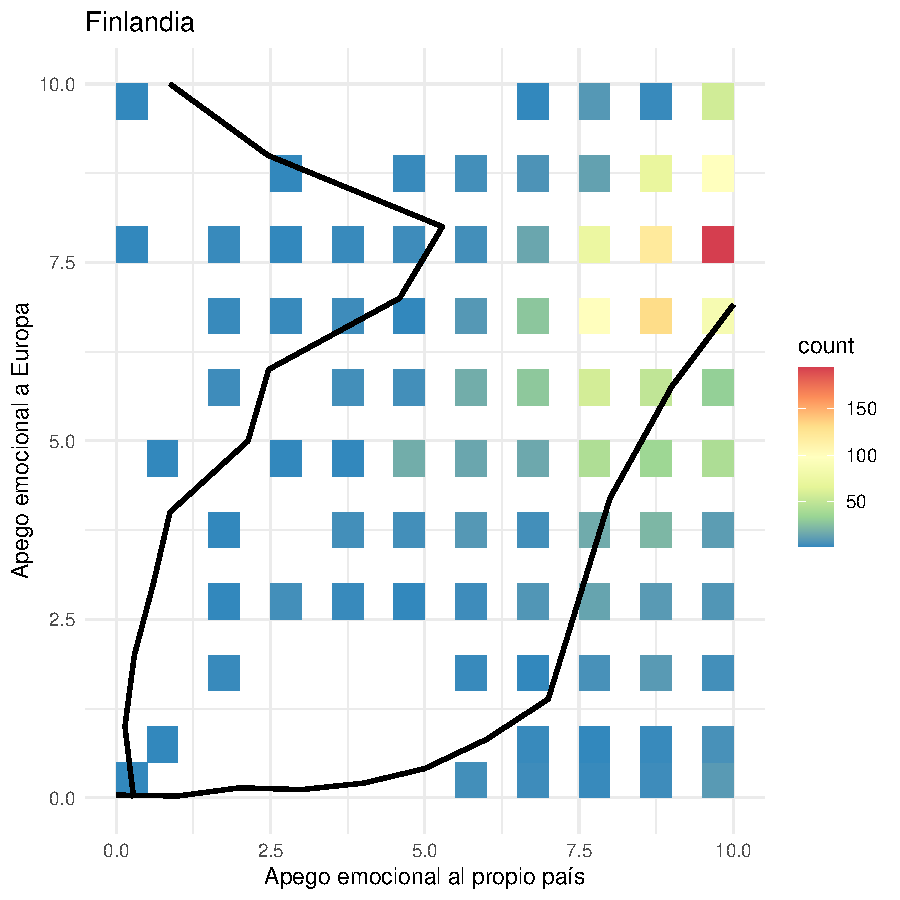
\includegraphics{Informe-017}

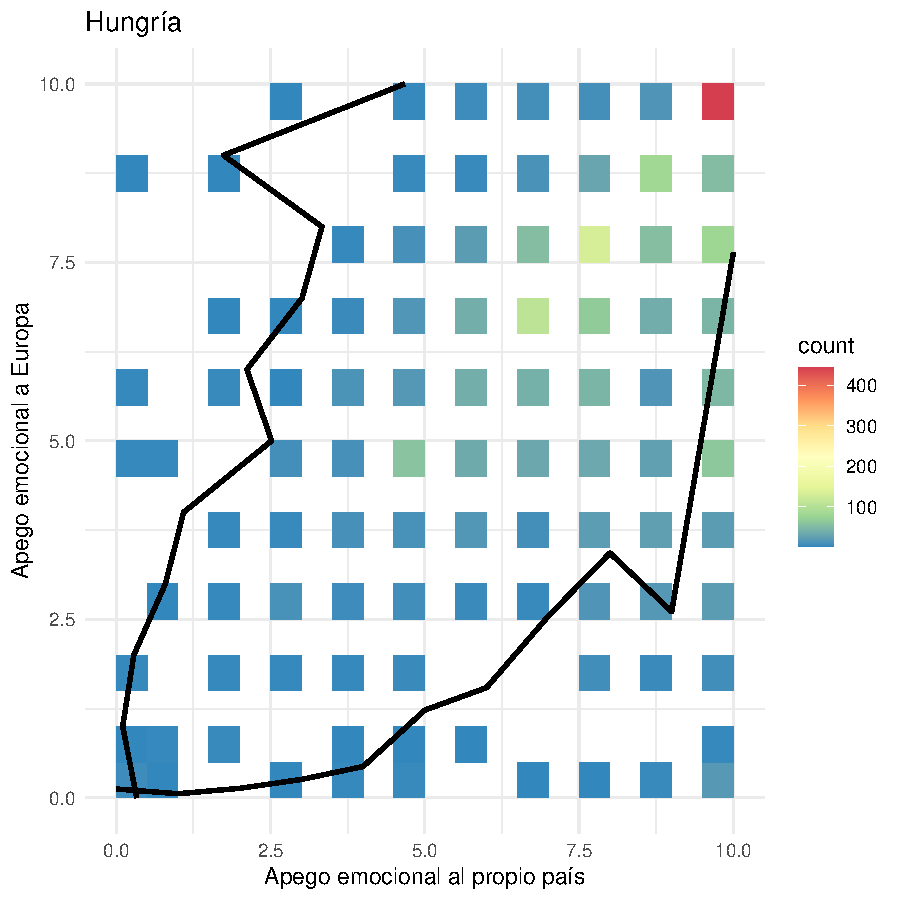
\includegraphics{Informe-018}

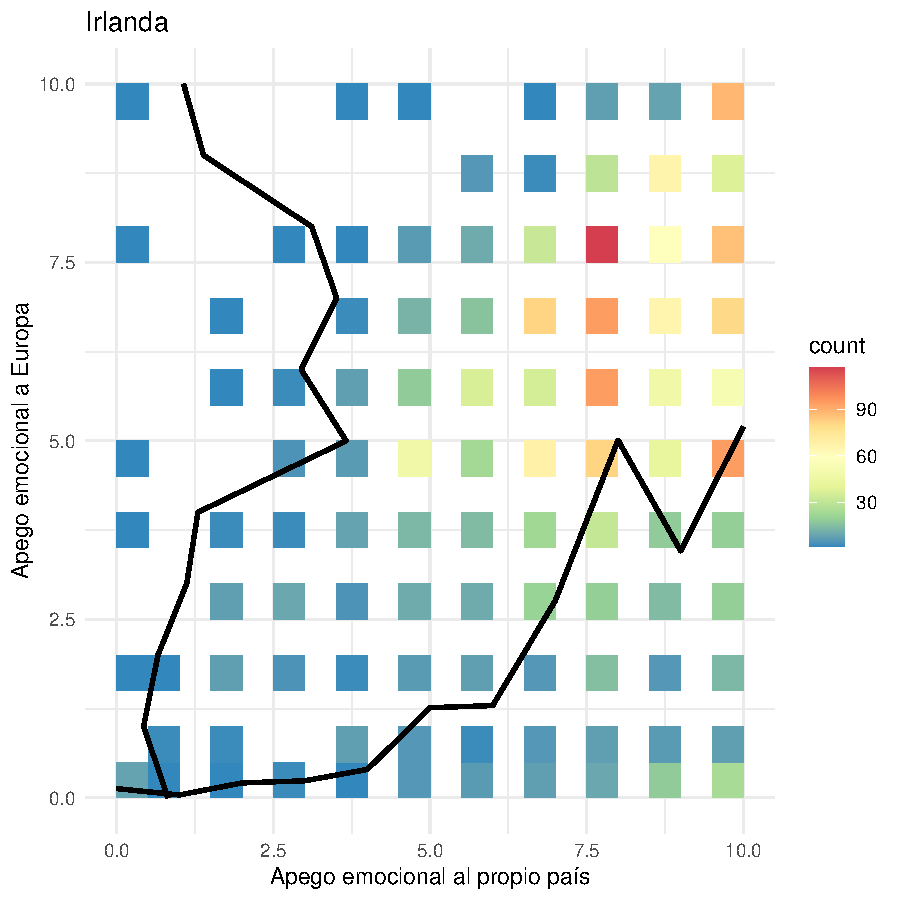
\includegraphics{Informe-019}

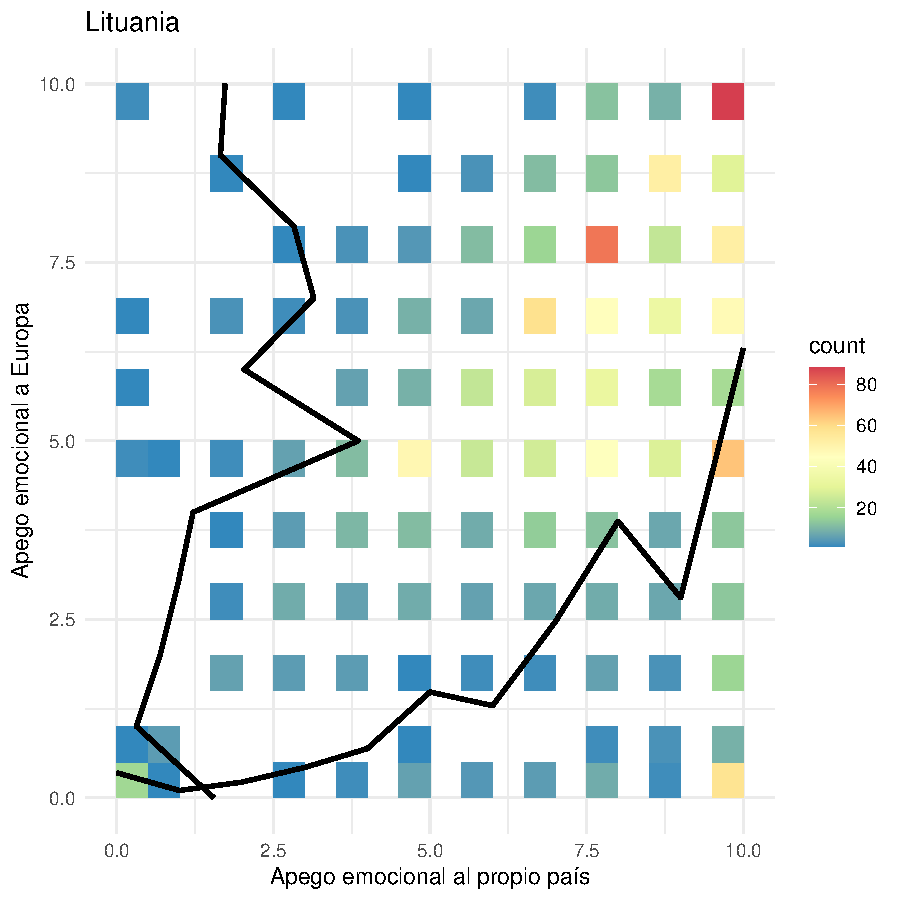
\includegraphics{Informe-020}

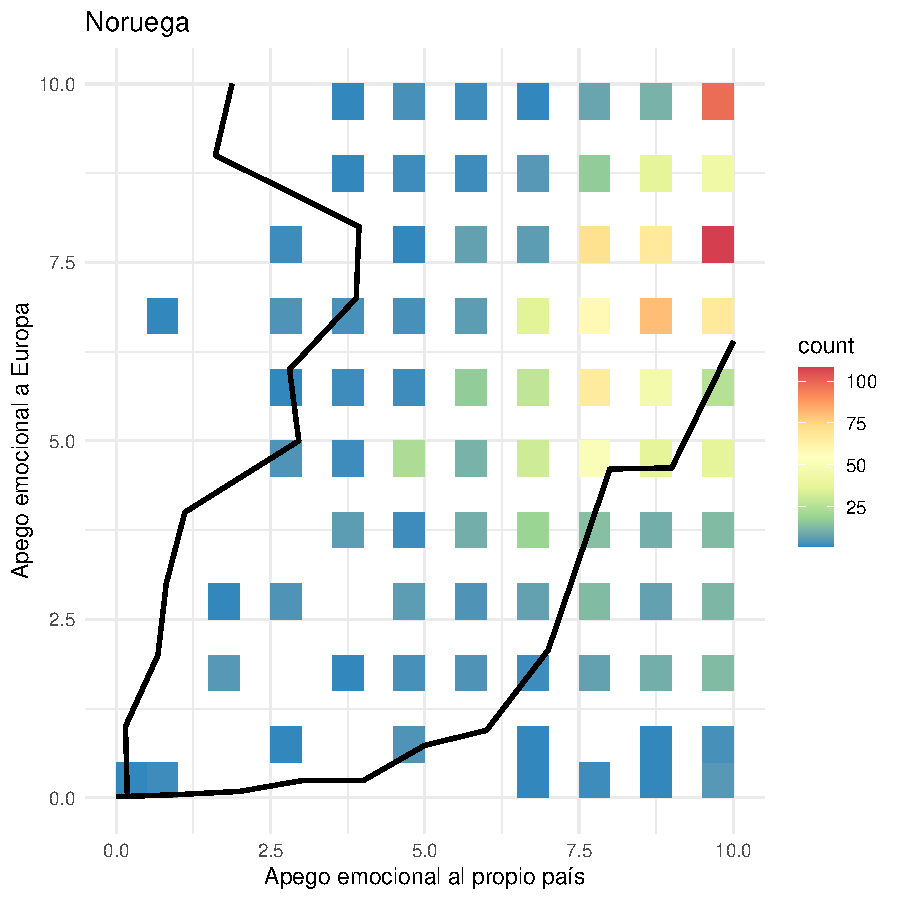
\includegraphics{Informe-021}

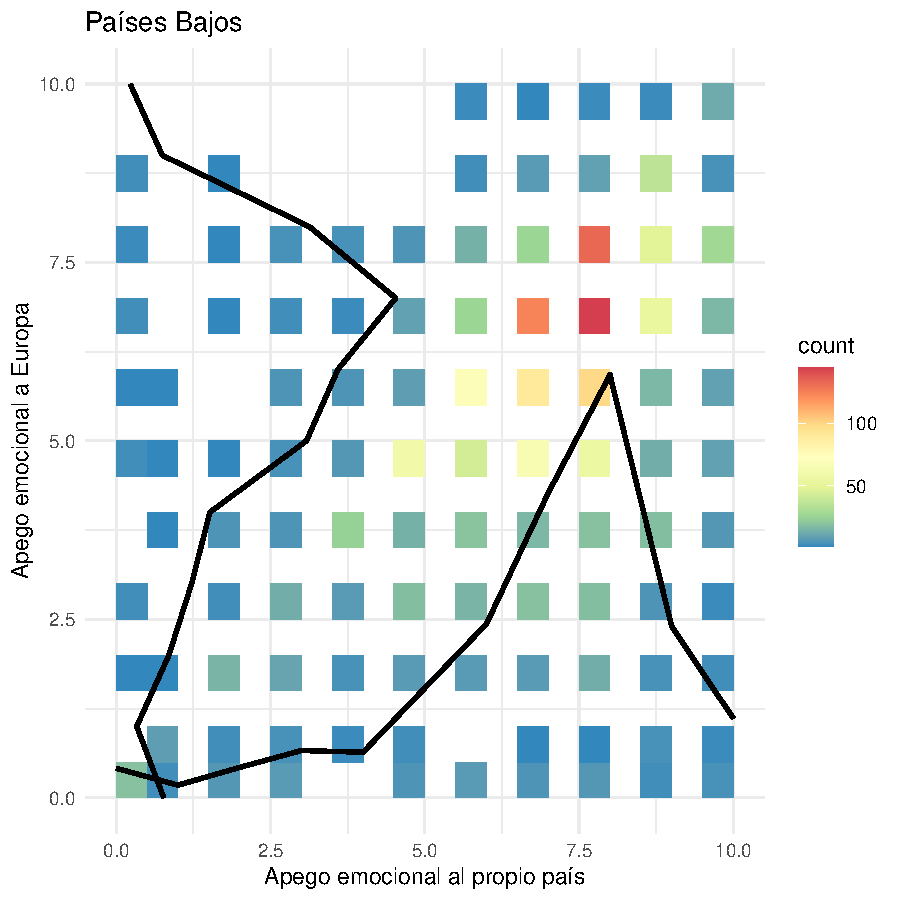
\includegraphics{Informe-022}

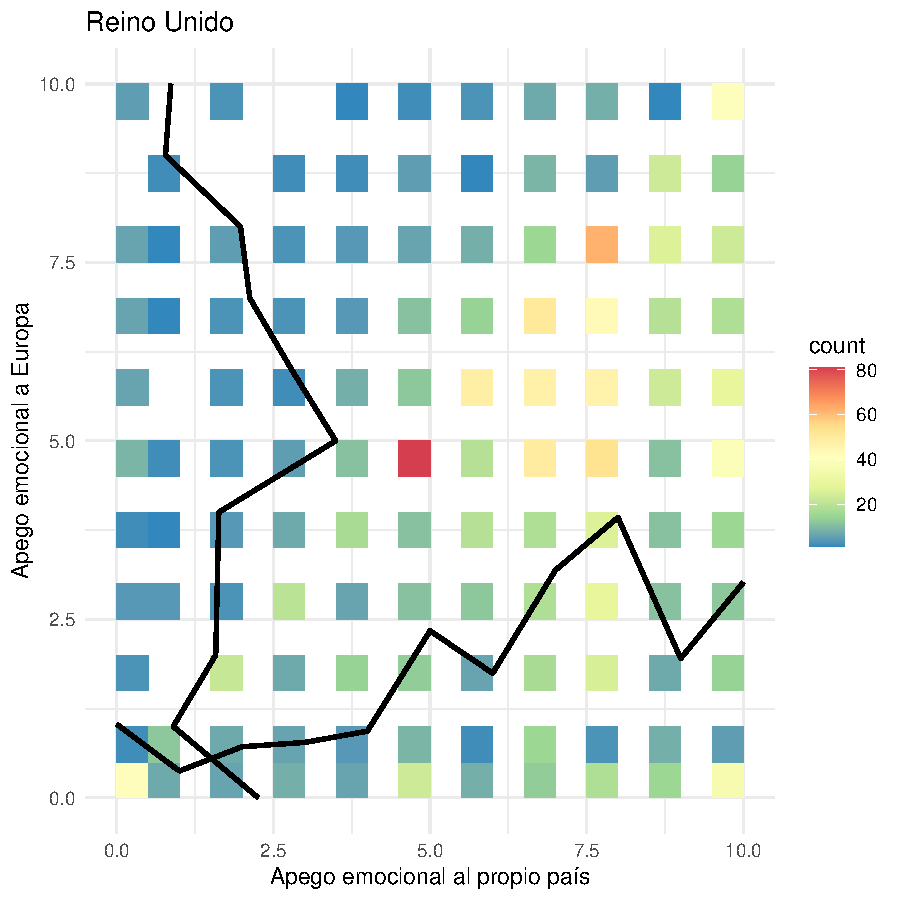
\includegraphics{Informe-023}

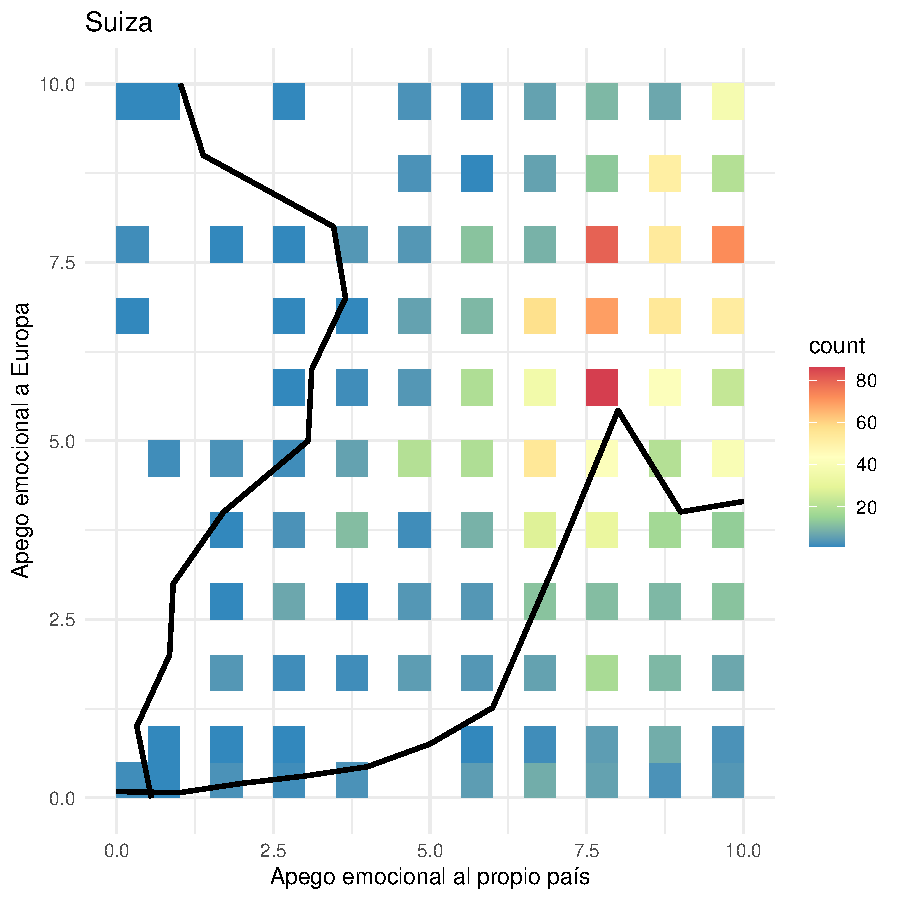
\includegraphics{Informe-024}

\newpage
\section{Estudiar y visualizar cómo correlacionan el apego emocional al propio país y el apego emocional a Europa entre diferentes subgrupos a escoger de entre los diferentes niveles de nuestras variables demográficas.}

\noindent El dashboard generado nos permite también visualizar todos los subconjuntos de muestras posibles de crear de entre todas las categorías de cada variable demográfica. Escogiendo una única categoría en cada variable demográfica podemos obtener un total de 130 submuestras diferentes.


\noindent Seguidamente mostramos la submuestra que presenta una correlación de Pearson mayor:
 \begin{figure}[H]
 \centering
 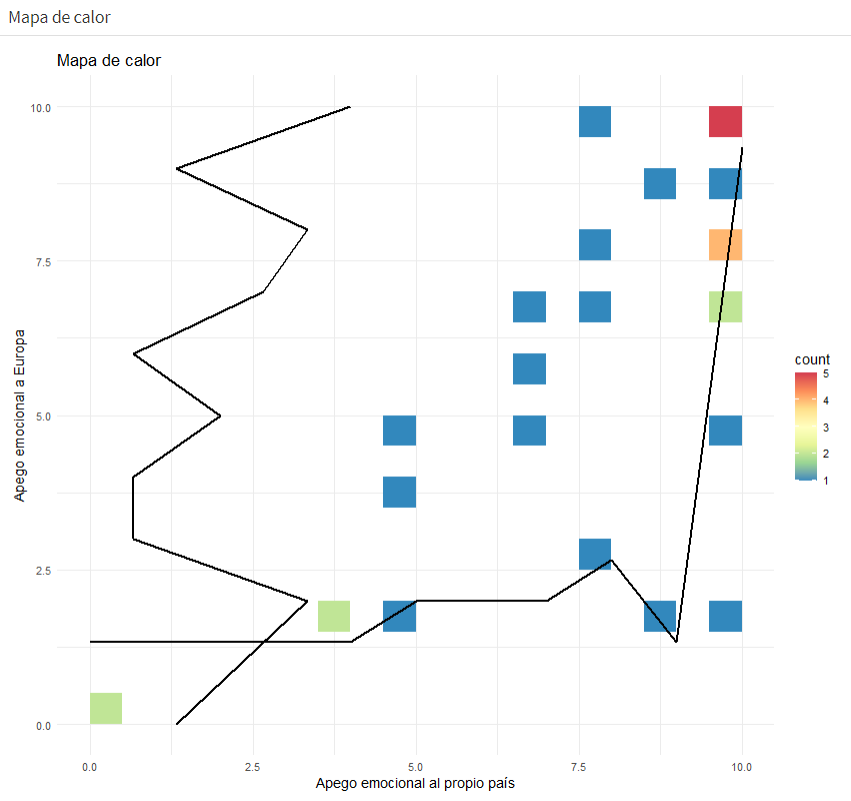
\includegraphics[width=0.7\textwidth]{Imatge1.png}
 \caption{Visualización de las correlaciones}
 \end{figure}
\noindent Dicha submuestra está compuesta por los hombres de 75 años o mayores de Lituania. La correlación que obtienen es de 0.7458912, claro que se trata de una muestra muy pequeña comparada con el total de observaciones de las que disponemos en la muestra total, y no es representativa.


\noindent Mostramos ahora la submuestra que presenta una correlación de Pearson menor:
 \begin{figure}[H]
 \centering
 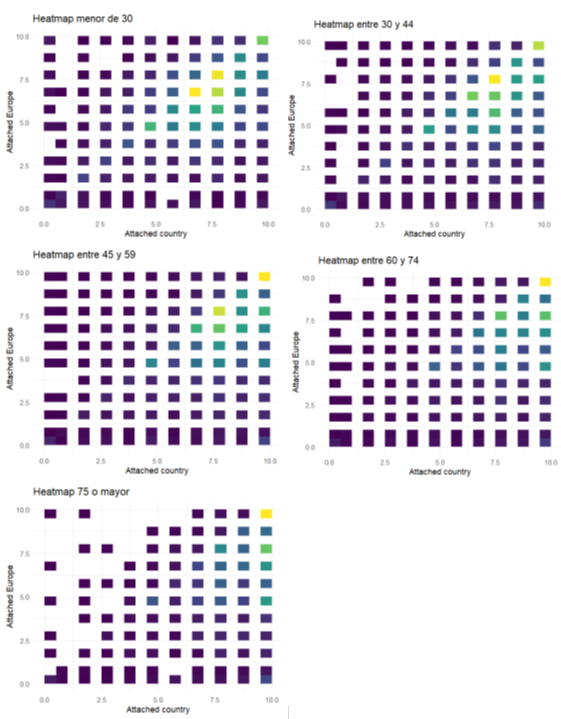
\includegraphics[width=0.7\textwidth]{Imatge2.png}
 \caption{Visualización de las correlaciones}
 \end{figure}
\noindent Dicha submuestra está compuesta por las mujeres de 75 años o mayores de Noruega. La correlación que obtienen es de 0.08331454, igualmente se trata de una muestra muy pequeña comparada con el total de observaciones, y tampoco es representativa.


\noindent El dashboard nos permite además escoger múltiples opciones de categorías de entre las variables demográficas. Esto resulta en una infinidad de opciones, el análisis de las cuales escapa los objetivos de este informe.

\newpage
\section*{Conclusiones}

\noindent Los resultados obtenidos en este informe nos permiten concluir que no se observan diferencias entre mujeres y hombres en la correlación de las variables 'Apego emocional al propio país' y 'Apego emocional a Europa', además los valores obtenidos en la correlación de Pearson nos permiten afirmar que no hay diferencias significativas en dicha correlación entre los hombres y mujeres que conforman nuestra muestra.


\noindent Por lo que hace a la variable demográfica 'edad' podemos observar que sí que influye en como se relacionan la variable de apego emocional al propio país y a Europa. Podemos observar cambios en qué nivel de apego tanto al país como a Europa son los más correlacionados. A medida que aumenta la edad, dicho nivel de correlación del apego entre el país y Europa se mueve desde valores moderados hasta los valores más elevados de apego. Los valores de la correlación que observamos en la tabla nos permiten ver como el rango de edad (o la generación) que obtiene una correlación menor es el rango de '75 o mayores' (0.3832552) y el rango que obtiene una correlación mayor es precisamente el rango de los más jóvenes 'menores de 30' (0.4800369). Tal y como observamos en los gráficos, la correlación de Pearson nos permite también concluir que en nuestra muestra a medida que aumenta la edad aumenta la correlación, con un estancamiento entre los 45 y los 70 años aproximadamente.


\noindent Por lo que hace a la variable demográfica 'nacionalidad' podemos observar que sí que influye en como se relacionan la variable de apego emocional al propio país y a Europa. Se pueden observar tanto cambios en la intensidad en como se correlacionan, como en qué nivel de apego tanto al país como a Europa son los más correlacionados. Vemos que hay un claro parecido de gráficos entre los países más occidentales, los más orientales y los escandinavos. Además, cabe destacar que el Reino Unido radicaliza la tendencia de los países más occidentales. Los países más occidentales tienden a presentar mayor correlación entre los valores moderados/altos pero no extremamente altos de la variable apego al propio país y los valores también moderados/altos pero no extremamente de la variable apego a Europa. Los países más orientales tienden a presentar mayor correlación entre los valores extremamente altos de la variable apego al propio país y los valores también extremamente altos de la variable apego a Europa. Finalmente, los países escandinavos tienden a presentar mayor correlación entre los valores extremamente altos de la variable apego al propio país y valores moderados/altos de la variable apego a Europa.


\noindent Los valores de la correlación de Pearson nos indican que el país con una correlación menor es Lituania (0.2824732) indicándonos que en este país el apego al propio país no predice tanto el apego a Europa (y a la inversa) como pasa en otros países. El país con una correlación mayor es Alemania (0.5506882) indicándonos que en este país el apego al propio país predice más el apego a Europa (y a la inversa) que en otros países.


\noindent Por lo que hace a los gráficos obtenidos a partir de la submuestra con una correlación de Pearson menor y la submuestra con la correlación mayor podemos concluir que el rango de valores de las correlaciones obtenidas en cada subconjunto de variables es muy ámplio. Aún así futuros estudios podrían observar con mayor precisón como es la distribución de las correlaciones entre cada posible submuestra compuesta por una única categoría de cada variable demográfica e incluso de las compuestas por más de una categoría, así como estudiar su representatividad. La información referente a las distribuciones de las dos variables de apego emocional que encontramos representada con una línea negra encima de los mapas de calor podría también interesante de analizar.

\end{document}
